\subsection{Gauss-Legendre Integration (Optional)}



\frame{
We wish to find the area under the curve 
\begin{equation*}
y = f(x) \ \ \ -1 \le x \le 1
\end{equation*}
\begin{center}
$\Downarrow$
\end{center}
\begin{block}{}
What method gives the best answer if only two function evaluations are to be made? 
\end{block}
}

\frame{
\begin{itemize}
\item The trapezoidal rule is a method for finding the area under the curve and that it uses two function evaluations at the endpoints $(-1, f ( -1))$, and ($1, f(1))$. 
\item But if the graph of $y = f(x)$ is concave down, the error in approximation is the entire region that lies between the curve and the line segment joining the points. 
\end{itemize}
\begin{figure}
\begin{center}
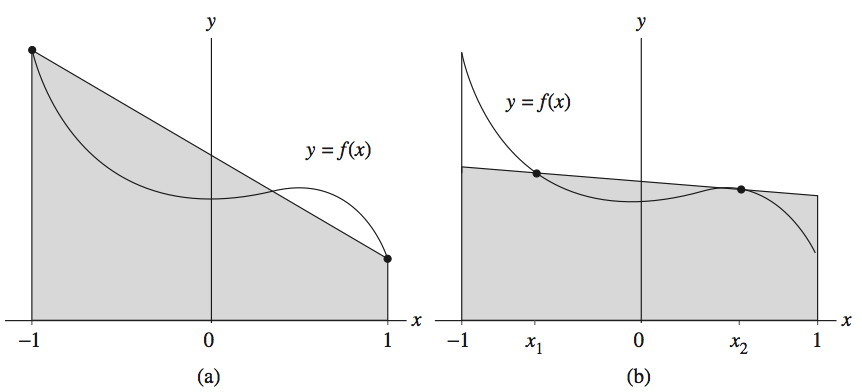
\includegraphics[width=100mm]{chap-5/fig_7-10.png}
\end{center}
\end{figure}
}

\frame{
If we can use nodes $x_1$ and $x_2$ that lie inside the interval $[-1,1]$, the line through the two points $(x_1, f(x_1))$ and $(x_2, f(x_2))$ crosses the curve, and the area under the line more closely approximates the area under the curve. 
\begin{center}
$\Downarrow$
\end{center}
The equation of the line is 
\begin{equation*}
y = f(x_1) + \frac{(x -x_1)\left( f(x_2)- f(x_1) \right)}{x_2 - x_1}
\end{equation*}
and the area of the trapezoid under the line is
\begin{equation*}
A_{trap} = \frac{2 x_2 }{x_2 - x_1} f (x_1) - \frac{ 2 x_1}{x_2 - x_1} f (x_2).
\end{equation*}
}

\frame{
When we choose $x_1 = -1$, $x_2 = 1$, and $h = 2$, then
\begin{equation*}
T ( f, h) = \frac{2}{2} f (x_1) - \frac{-2}{2} f (x_2) = f (x1) + f (x2) .
\end{equation*}
\begin{figure}
\begin{center}
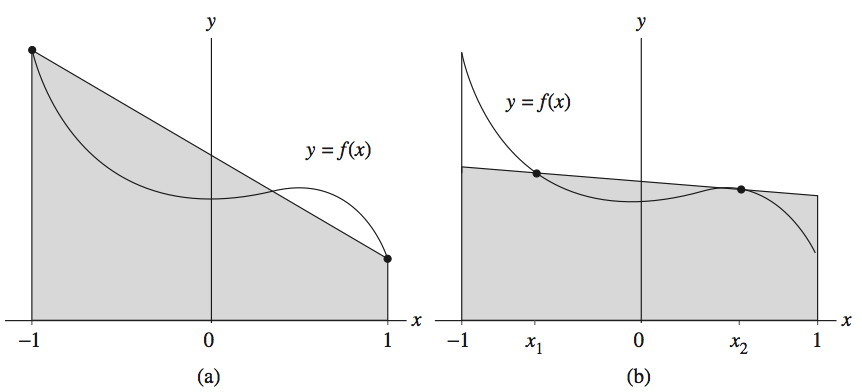
\includegraphics[width=100mm]{chap-5/fig_7-10.png}
\end{center}
\end{figure}
}

\frame{
We shall use the method of undetermined coefficients to find the abscissas $x_1$, $x_2$ and weights $w_1$, $w_2$ so that the formula 
\begin{equation*}
\int_{-1}^{1} f(x) d x \approx w_1 f(x_1) + w_2 f(x_2)
\end{equation*}
is exact for cubic polynomials\footnote{ i.e., $f(x) = a_3x^3 + a_2x^2 + a_1x + a_0$}. 
\begin{center}
$\Downarrow$
\end{center}
\begin{itemize}
\item Since four coefficients $w_1$, $w_2$, $x_1$, and $x_2$ need to be determined in the equation, we can select four conditions to be satisfied. 
\item Using the fact that integration is additive, it will suffice  to require that the equationbe exact for the four functions $f(x) = 1, x, x^2, x^3$. 
\end{itemize}
}

\frame{
The four integral conditions :
\begin{block}{}
\begin{equation*}
\begin{array}{l l}
f(x) = 1 : & \int_{-1}^1 dx = w_1 + w_2 \\
& \\
f(x) = x : & \int_{-1}^1 x dx = 0 = w_1 x_1 + w_2 x_2 \\
& \\
f(x) = x^2 : & \int_{-1}^1 x^2 dx = w_1 x_1^2 + w_2 x_2^2 \\
& \\
f(x) = x^3 : & \int_{-1}^1 x^3 dx = 0 = w_1 x_1^3 + w_2 x_2^3 \\
\end{array}
\end{equation*}
\end{block}
}

\frame{
Solve the system of nonlinear equations 
\begin{equation*}
\begin{array}{r l}
w_1 + w_2  & = 2 \\
w_1 x_1 & = -w_2 x_2 \\
w_1^2 + w_2^2 & = \frac{2}{3}\\
w_1 x_1^3 & = -w_2 x_2^3
\end{array}
\end{equation*}
\begin{center}
$\Downarrow$
\end{center}
We can divide the forth by the second of the above equations and the result is 
\begin{equation*} 
x_1^2 = x_2^2 \ \ or \ \ x_1 = -x_2
\end{equation*}
}

\frame{
Use the above equations, we can get 
\begin{equation*}
w_1 = w_2
\end{equation*}
Using the above results in $w_1 + w_2 = 2$.
Hence
\begin{equation*}
w_1 = w_2 = 1
\end{equation*}
\begin{center}
$\Downarrow$
\end{center}
We can write
\begin{equation*}
w_1 x_1^2 + w_2 x_2^2 = x_2^2 + x_2^2 = \frac{2}{3} \ \ \ or \ \ \ x_2^2 = \frac{1}{3}
\end{equation*}
}

\frame{
Finally,  the nodes are 
\begin{equation*}
-x_1 = x_2 = 1 \slash 3^{1\slash2} \approx 0.5773502692.
\end{equation*}
\vspace{0.3cm}
\begin{block}{}
\begin{itemize}
\item We have found the nodes and weights that make up the two-point Gauss-Legendre rule. 
\vspace{0.3cm}
\item Since the formula is exact for cubic equations, the error term will involve the fourth derivative. 
\end{itemize}
\end{block}
}

\frame{
\begin{block}{Theorem  (Gauss-Legendre Two-Point Rule).}
If $f$ is continuous on $[-1, 1]$, then
\begin{equation*}
\int_{-1}^{1} f(x) dx \approx G_2 (f) = f \left( \frac{-1}{\sqrt{3}} \right) + f \left( \frac{1}{\sqrt{3}} \right)
\end{equation*}
The Gauss-Legendre rule $G_2( f )$ has degree of precision $n = 3$. 
If $f \in C^4 [-1, 1]$,
\begin{equation*}
\int_{-1}^{1} f(x) dx = f \left( \frac{-1}{\sqrt{3}} \right) + f \left( \frac{1}{\sqrt{3}} \right) + E_2(f)
\end{equation*}
where
\begin{equation*}
E_2(f) = \frac{f^{(4)}(c)}{135}
\end{equation*}
\end{block}
}

\frame{
\begin{block}{Example}
Use the two-point Gauss-Legendre rule to approximate
\begin{equation*}
\int_{-1}^1 \frac{dx}{x+2} = \ln(3) - \ln(1) \approx 1.09861
\end{equation*}
and compare the result with the trapezoidal rule $T ( f, h)$ with $h = 2$ and Simpson’s rule $S( f, h)$ with $h = 1$.
\end{block}
Let $G_2( f )$ denote the two-point Gauss-Legendre rule; then
\begin{equation*}
\begin{array}{r l}
G_2( f ) & = f (-0.57735) + f (0.57735) \\
& \\
& = 0.70291 + 0.38800 = 1.09091,
\end{array}
\end{equation*}
}

\frame{
\begin{equation*}
\begin{array}{r l}
T ( f, 2) & = f (-1.00000) + f (1.00000) \\
& \\
& = 1.00000 + 0.33333 = 1.33333, \\
& \\
S(f,1) & = \frac{f(-1)+4f(0)+ f(1)}{3}= \frac{1 + 2 + \frac{1}{3}}{3} \\
& \\
& = 1.11111.
\end{array}
\end{equation*}
The errors are $0.00770$, $-0.23472$, and $-0.01250$, respectivcly, so the Gauss-Legendre rule is seen to be best. 
}

\frame{
\begin{itemize}
\item Notice that the Gauss-Legendre rule required only two function evaluations and Simpson's rule required three. 
\item The size of the error for $G_2(f)$ is about $61\%$ of the size of the error for $S(f, 1)$. 
\end{itemize}
\begin{center}
$\Downarrow$
\end{center}
The general N-point Gauss-Legendre rule is exact for polynomial functions of degree $\le 2N - 1$, and the numerical integration formula is
\begin{equation*}
G_N(f)=w_{N,1} f(x_{N,1})+w_{N,2} f(x_{N,2})+ \cdots + w_{N,N} f(x_{N,N}).
\end{equation*}
}

\frame{
\begin{itemize}
\item The abscissas $x_{N,k}$ and weights $w_{N,k}$ to be used have been tabulated and are easily available and the table  gives the values up to eight points. 
\item Also included in the table is the form of the error term $E_N(f)$ that corresponds to $G_N(f)$, and it can be used to determine the accuracy of the Gauss-Legendre integration formula. 
\end{itemize}
\begin{figure}
\begin{center}
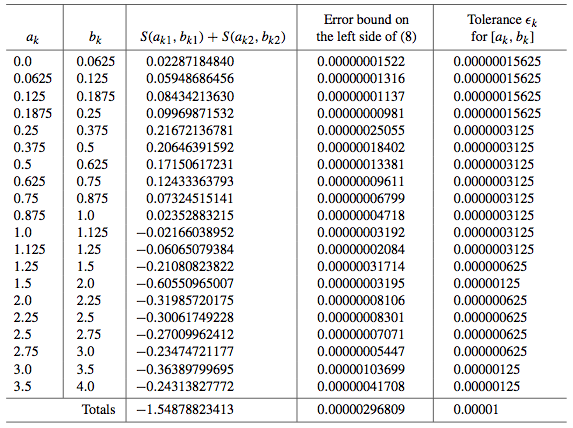
\includegraphics[width=80mm]{chap-5/tab_7-8.png}
\end{center}
\end{figure}
}

\frame{
\begin{itemize}
\item The values in Table \footnote{in the previous slide} in general have no easy representation. 
\item This fact makes the method less attractive for humans to use when hand calculations are required. 
\item But once the values are stored in a computer it is easy to call them up when needed. 
\item The nodes are actually roots of the Legendre polynomials, and the corresponding weights must be obtained by solving a system of equations.
\item For the three-point Gauss-Legendre rule the nodes are $-(0.6)^{1/2}$, $0$, and $(0.6)^{1/2}$, and the corresponding weights are $5/9$, $8/9$, and $5/9$. 
\end{itemize}
}

\frame{
\begin{block}{Theorem (Gauss-Legendre Three-Point Rule).}
If $f$ is continuous on $[-1, 1]$, then
\begin{equation*}
\int_{-1}^1 f(x) dx \approx G_3(f) = \frac{ 5 f(-\sqrt{3\slash5}) + 8 f(0) + 5 f(\sqrt{3 \slash 5})}{9}
\end{equation*}
The Gauss-Legendre rule $G_3( f )$ has degree of precision $n = 5$.  \\
If $f \in C^6[-1, 1]$, then
\begin{equation*}
\int_{-1}^1 f(x) dx  = \frac{5f(-\sqrt{3\slash5}) + 8f(0) + 5f(\sqrt{3\slash5})}{9} + E_3(f)
\end{equation*}
where
\begin{equation*}
E_3 (f) = \frac{f^{(6)}(c)}{15,750}
\end{equation*}
\end{block}
}

\frame{
\begin{block}{Example}
Show that the three-point Gauss-Legendre rule is exact for
\begin{equation*}
\int_{-1}^1 5 x^4 dx = 2 = G_3(f)
\end{equation*}
\end{block}
Since the integrand is $f (x) = 5x^4$ and $f (6)(x) = 0$, 
we can use the third equation \footnote{theorem 5.10}  to see that $E_3( f ) = 0$. 
But it is instructive to use the first equation and do the calculations in this case.
\begin{equation*}
G_3 (f) = \frac{5(5)(0.6)^2 + 0 + 5(5)(0.6)^2}{9} = \frac{18}{9} = 2
\end{equation*}
}

\frame{
\begin{block}{Theorem (Gauss-Legendre Translation).}
Suppose that the abscissas $\{ x_{N,k}\}^N_{k=1}$ and weights $\{w_{N,k}\}^N_{k=1}$ are given for the $N-$point Gauss-Legendre rule over $[-1,1]$. 
To $k=1$ apply the rule over the interval $[a, b]$, use the change of variable
\begin{equation*}
t = \frac{a+b}{2} + \frac{b-a}{2} x \ \ \  and \ \ \ dt = \frac{b-a}{2} dx
\end{equation*}
Then the relationship
\begin{equation*}
\int_a^b f(t) dt = \int_{-1}^{1} f\left( \frac{a+b}{2} + \frac{b-a}{2} x \right) \frac{b-a}{2} dx
\end{equation*}
is used to obtain the quadrature formula
\begin{equation*}
\int_a^b f(t) dt = \frac{b-a}{2} \sum_{k=1}^N w_{N,k}  f \left( \frac{a+b}{2} + \frac{b-a}{2} x_{N,k} \right) 
\end{equation*}
\end{block}
}

\frame{
\begin{block}{Example.}
Use the three-point Gauss-Legendre rule to approximate
\begin{equation*}
\int_1^5 \frac{dt}{t} = \ln(5) -\ln(1) \approx 1.609438
\end{equation*}
and compare the result with Boole’s rule $B(2)$ with $h = 1$.
\end{block}
Here $a = 1$ and $b = 5$, so the rule in theorem 5.11 yields
\begin{equation*}
\begin{array}{r l}
G_3(f) & = (2) \frac{5 f (3 - 2(0.6)^{1\slash2}) + 8 f (3 + 0) + 5 f (3 + 2(0.6)^{1\slash2})}{9}\\
& \\
 & = (2) \frac{3.446359 + 2.666667 + 1.099096}{9} = 1.602694.\\
\end{array}
\end{equation*}
}

\frame{
\begin{itemize}
\item In the example we saw that Boole's rule gave $B(2) = 1.617778$. 
\item The errors are $0.006744$ and $-0.008340$, respectively, so that the Gauss-Legendre rule is slightly better in this case. 
\item Notice that the Gauss-Legendre rule requires three function evaluations and Boole's rule requires five. 
\item In this example the size of the two errors is about the same. 
\end{itemize}
}

\frame{
\begin{itemize}
\item Gauss-Legendre integration formulas are extremely accurate, and they should be considered seriously when many integrals of a similar nature are to be evaluated. 
\item In this case, proceed as follows. 
\begin{itemize}
\item Pick a few representative integrals, including some with the worst behavior that is likely to occur. 
\item Determine the number of sample points $N$ that is needed to obtain the required accuracy. 
\item Then fix the value $N$, and use the Gauss-Legendre rule with $N$ sample points for all the integrals. 
\end{itemize}
\end{itemize}
}

%\frame{
%\begin{itemize}
%\item For a given value of $N$, Program 5.7 requires that the abscissas and weights from Table 5.8 be saved in $1 \times N$ matrices $A$ and $W$, respectively. 
%\item This can be done in the MATLAB command window or the matrices can be saved as M-files. 
%\item It would be expedient to save Table 5.8 in a $35 \times 2$ matrix $G$. 
%\item The first column of $G$ would contain the abscissas and the second column the corresponding weights. 
%\item Then, for a given value of $N$, the matrices $A$ and $W$ would be submatrices of $G$. 
%\item For example, if $N = 3$, then $A=G(3:5,1)'$ and $W=G(3:5,2)'$. 
%\end{itemize}
%}

